\documentclass[times, utf8, diplomski]{fer}
\usepackage{booktabs}
\usepackage{graphics}
\usepackage{algorithm}
\usepackage{algorithmic}
\usepackage{caption}
\usepackage{listings}
\usepackage{natbib}
\usepackage{xcolor}
\usepackage{hyperref}
\usepackage{subcaption}
\usepackage{graphicx}
\usepackage{float}

\urlstyle{same}

% Citiranje oznaceno brojevima
\setcitestyle{numbers}

% Da ispod programskih isjecaka pise Isjecak umjesto Listing
\renewcommand{\lstlistingname}{Isječak}% Listing -> Isječak
% \renewcommand{\lstlistlistingname}{Lista \lstlistingnamea}% List of Listings -> Lista Isječaka

% Boje za programski kod
\definecolor{codegreen}{rgb}{0,0.35,0}
\definecolor{codegray}{rgb}{0.5,0.5,0.5}
\definecolor{codeblue}{rgb}{0.3, 0.6, 1}
\definecolor{codeorange}{rgb}{0.9, 0.45, 0}
\definecolor{backcolour}{rgb}{0.95,0.95,0.92}

%style za programski kod imena "mystyle"
\lstdefinestyle{mystyle}{
  backgroundcolor=\color{backcolour}, commentstyle=\color{codegreen},
  keywordstyle=\color{codeblue},
  numberstyle=\tiny\color{codegray},
  stringstyle=\color{codeorange},
  basicstyle=\ttfamily\scriptsize,
  breakatwhitespace=false,         
  breaklines=true,                 
  captionpos=b,                    
  keepspaces=true,                 
  numbers=left,                    
  numbersep=5pt,                  
  showspaces=false,                
  showstringspaces=false,
  showtabs=false,                  
  tabsize=1,
}

%"mystyle" code listing set
\lstset{style=mystyle}

\begin{document}

\thesisnumber{2493}

\title{Modeli za generiranje trodimenzionalnih objekata}

\author{Bruno Sačarić}

\maketitle

% Ispis stranice s napomenom o umetanju izvornika rada. Uklonite naredbu \izvornik ako želite izbaciti tu stranicu.
\izvornik

% Dodavanje zahvale ili prazne stranice. Ako ne želite dodati zahvalu, naredbu ostavite radi prazne stranice.
\zahvala{

Zahvaljujem asistentima mag. ing. Luki Posiloviću i mag. ing. Duji Medaku na suradnji, savjetima, strpljenju i profesionalnom odnosu. Zahvaljujem bratu i roditeljima za potporu i što su mi omogućili da se posvetim studiranju. Zahvaljujem Anji što je bila uz mene u izradi ovog rada.}

\tableofcontents

\chapter{Uvod}
%- što je zadatak (problem)
%- zašto ga rješavamo (motivacija)
%- kako ga rješavamo (pristup)
%- opis organizacije ostatka dokumenta(najčešće po poglavljima)
%- obično ne više od 1 stranice

Računarstvo nam kroz svoje primjene omogućuje da iskoristimo potencijal digitalnih strojeva za rješavanje složenih problema, obradu podataka, simulaciju i analizu sustava te delegiranje poslova kako bi poboljšali vlastite živote i pronašli odgovore na mnoga pitanja. Umjetna inteligencija kao područje računarstva se bavi razvojem sustava koji više ili manje samostalno uče obrađivati podatke temeljem iskustva i podataka. Trenutno se algoritmi umjetne inteligencije najčešće koriste za klasifikaciju ili prepoznavanje uzoraka u podacima, dakle izvlače znanje iz obilja informacija koje im damo te su \textit{diskriminatorne} prirode. Tema ovog rada su \textit{generativni} modeli dubokih neuronskih mreža koji pokušavaju, kroz obradu podataka, generirati nove, do sad neviđene podatke. Naši digitalni strojevi polako postaju sve bolji u generiranju, odnosno \textit{kreiranju}.

Pomoću tih modela pokušat ćemo naučiti sustave za generiranje trodimenzionalnih objekata u obliku voksela kako bismo bolje naučili algoritme za detekciju pukotina u materijalima. Na sustavu Google Colab pokrećemo programe kako bi iskoristili hardverske resurse dostupne u Google-ovim podatkovnim centrima te značajno skratili vrijeme učenja mreže.

U 2. poglavlju dani su osnovni pojmovi dubokog učenja. U 3. poglavlju je predstavljen model generativne suparničke mreže i navedene su neke njegove novije vrste. 4. poglavlje predstavlja 3DGAN mrežu, dok je u 5. poglavlju dana njena implementacija. 6. poglavlje prezentira rezultate učenja mreže.

\chapter{Duboko učenje}
\section{Uvod u duboko učenje}
Duboko učenje područje je umjetne inteligencije usredotočeno na stvaranje velikih modela neuronskih mreža, sposobnih \textit{donositi valjane odluke temeljem dostupnih podataka}. Ono je posebice primjereno situacijama masivnih skupova podataka, napučenih složenim podacima. Duboko učenje omogućuje \textit{odlučivanje na temelju podataka}, pronalaženjem i izdvajanjem uzoraka podataka iz velikih skupova podataka, koji se precizno preslikavaju u valjane izlazne odluke. \cite{knjiga}

Mreža dubokog učenja matematički je model koji je nadahnut strukturom mozga. U svom najjednostavnijem obliku, matematički model je jednadžba koja opisuje način koji jednu ili više ulaznih varijabli povezuje s izlaznom varijablom. U ovom obliku, matematički je model isto što i funkcija - preslikavanje ulaza u izlaz. \cite{knjiga}

Duboko učenje nastalo je iz istraživanja umjetne inteligencije i strojnog učenja. Strojno učenje uključuje razvoj i vrednovanje algoritama koji računalu omogućavaju izvlačenje (ili učenje) funkcija iz skupa podataka (skupa primjera) pomoću neke funkcije. \cite{knjiga} \\

\begin{figure}
\centering
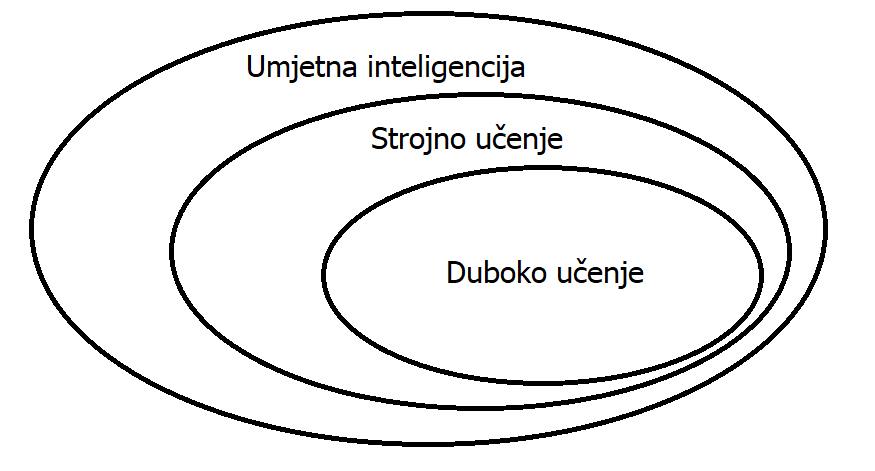
\includegraphics[scale=0.55]{Duboko učenje.png}   
\caption{Vennov dijagram Umjetne inteligencije}
\end{figure}

\break

%Pojam \textit{duboko učenje} opisuje obitelj modela \textit{neuronskih mreža} s više slojeva jednostavnih programa za obradu informacija, poznatih kao neuroni. Neuronska mreža je računski model inspiriran strukturom ljudskog mozga. Ljudski mozak sastoji se od golemog broja živčanih stanica, zvanih neuroni. \cite{knjiga}

%Umjetna neuronska mreža sastoji se od mreže jednostavnih jedinica za obradu informacija, zvanih neuroni. Snaga neuronskih mreža u pogledu modeliranja složenih odnosa nije rezultat složenih matematičkih modela, već proizlazi iz interakcija velikog skupa jednostavnih neurona.\cite{knjiga}

%Slika prikazuje strukturu neuronske mreže. Neuroni u neuronskoj mreži organizirani su u slojeve. Prikazana mreža ima pet slojeva: jedan ulazni sloj, tri skrivena sloja i jedan izlazni sloj. Mreže dubokog učenja su neuronske mreže koje imaju mnogo skrivenih slojeva neurona, a minimalni broj skrivenih slojeva potrebnih za razmatranje dubokih mreža je dva.\cite{knjiga}

\section{Neuronske mreže}
Pojam \textit{duboko učenje} opisuje obitelj modela mreža s više slojeva jednostavnih programa za obradu informacija, izvorno nazvanih perceptroni. Perceptron je osmišljen kao stroj koji predstavlja pojednostavljeni biološki neuron. Višeslojni perceptron je time pojednostavljeni model biološkog mozga, danas poznatiji kao \textit{neuronska mreža}. \cite{perceptron}

Umjetna neuronska mreža u svojem osnovnom obliku sastoji se od slojeva tih jednostavnih programskih jedinica, zvanih neuroni. Snaga neuronskih mreža u pogledu modeliranja složenih odnosa nije rezultat složenih matematičkih modela, već proizlazi iz interakcija velikog skupa neurona. \cite{knjiga}

Slika 2.2 prikazuje strukturu jedne neuronske mreže. Neuroni prikazane neuronske mreže organizirani su u pet slojeva: jedan ulazni sloj, tri skrivena sloja i jedan izlazni sloj. Mreže dubokog učenja su neuronske mreže koje obično imaju mnogo skrivenih slojeva, a minimalni broj skrivenih slojeva potrebnih za razmatranje dubokih mreža je dva. \cite{knjiga} \\

\begin{figure}[h]
\centering
\includegraphics[scale=0.55]{Neuronska mreža.png}
\caption{Struktura neuronske mreže}
\end{figure}

Svaka od veza u mreži ima s njom povezanu težinu. Težina veze jednostavno je broj, ali vrlo važan. Težina veze utječe na to kako neuron obrađuje informacije koje mu kroz nju pristižu, i zapravo, učenje umjetne neuronske mreže u suštini se svodi na traženje najboljeg skupa težina. Neuron, temeljni gradivni blok neuronskih mreža i dubokog učenja, definiran je jednostavnim slijedom dvaju koraka: računanjem težinskog zbroja u prvom i njegovom prosljeđivanju aktivacijskoj funkciji u drugom. \cite{knjiga}

\section{Konvolucijske neuronske mreže}
Konvolucijske neuronske mreže (CNN\footnote{Engl. Convolutional Neural Network}) oblikovane su za zadaće prepoznavanja slika i izvorno primijenjene na problem prepoznavanja rukom napisanih znamenki. Osnovni cilj dizajna CNN-a bio je stvaranje mreže u kojoj će neuroni u njezinim ranim slojevima izvlačiti lokalne vizualne značajke, a oni u kasnijima kombinirati ove značajke kako bi stvorili značajke višeg reda. Na primjer, kad se primijene na zadaću prepoznavanja lica, neuroni u ranijim slojevima CNN-a nauče se aktivirati kao odgovor na jednostavne lokalne značajke (poput linija pod određenim kutom ili segmenata krivulja), dok neuroni u završnim slojevima mreže kombiniraju aktivacije dijelova tijela kako bi na slici tijela mogli prepoznati lice. Sukladno ovom pristupu, osnovna zadaća prepoznavanja slike jest učenje funkcija otkrivanja značajki koje na jasan način mogu prepoznati prisutnost ili odsutnost lokalnih vizualnih značajki na slici. \cite{knjiga}

\section{Budućnost dubokog učenja}
Duboko učenje idealno je za aplikacije koje uključuju velike skupove visokodimenzionalnih podataka. Prema tome, ono će vjerojatno značajno pridonijeti nekima od glavnih znanstvenih izazova našeg doba. Što su neuronske mreže složenije, to ih se duže trenira i teže koristi pa se u prošlosti nisu toliko koristile, ali u današnje doba jakih računala, koriste se sve više. U posljednja dva desetljeća, proboj u tehnologiji biološkog sekvenciranja omogućio je stvaranje visoko preciznih sekvenci DNK. Ovi genetski podaci mogu biti temelj za sljedeću generaciju personalizirane precizne medicine. Istovremeno, međunarodni istraživački projekti, poput akceleratora čestica \textit{Large Hadron Collider} ili brojnih teleskopa u Zemljinoj orbiti, svakodnevno generiraju goleme količine podataka. Analiza tih podataka može pomoći razumjeti fiziku našeg svemira u rasponu od najmanjih do najvećih mjerila. Kao odgovor na ovu poplavu podataka, znanstvenici se u sve većem broju okreću strojnom i dubokom učenju, koji bi im omogućili analizu svih tih podataka. \cite{knjiga}

\chapter{Generativne suparničke mreže - GAN}
\section{Generativni modeli}
Generativni modeli nastoje naučiti raspodjelu podataka (ili modelirati postupak koji ih je generirao). Često se koriste kako bi se naučila korisna reprezentacija podataka prije podučavanja nadgledanog modela. Generativne suparničke mreže (GAN\footnote{Engl. Generative Adversarial Networks}) pristup su obučavanju generativnih modela koji je posljednjih godina polučio veliku pozornost. \cite{knjiga}

GAN se sastoji od dvije neuronske mreže, generativnog modela i diskriminativnog modela te uzorka stvarnih podataka. Modeli se obučavaju na suparnički (oponentski, suprotstavljeni, kontradiktorni) način. Zadaća diskriminativnog modela je naučiti razlikovati stvarne podatke - iz skupa podataka, i lažne podatke - stvorene generatorom. Zadaća generatora je naučiti stvarati lažne podatke koji će zavarati diskriminativni model. \cite{knjiga}

Generativni modeli obučeni pomoću GAN-ova mogu naučiti stvarati lažne slike koje oponašaju određeni umjetnički stil, kao i medicinske slike s oznakama ozljeda. Učenje stvaranja medicinskih slika, uz segmentaciju ozljeda na njima, otvara mogućnost automatskog generiranja masovnih skupova označenih slika koje se mogu koristiti za nadzirano učenje. Zabrinjavajuća primjena GAN-ova je stvaranje tzv. dubokih falsifikata \engl{deep fake} kao na primjer lažni videozapis osobe koja čini nešto što nikad nije činila, stvoren umetanjem njezina lika u videozapis nekoga drugoga. Duboke laži vrlo je teško otkriti i već su više puta zlonamjerno korištene za sramoćenje javnih osoba i širenje lažnih vijesti. \cite{knjiga}
\vfill

\section{Tipovi GAN-ova}
\addtocontents{toc}{\protect\setcounter{tocdepth}{2}}
\subsubsection{SRGAN – Super Resolution GANs}
U filmovima često viđamo kako neki informatičar uvećava mutnu fotografiju snimljenu kamerom, izoštrava je i pokazuje nam zlikovca. Na sličan način, SRGAN se trenira tako da može generirati realistične fotografije visoke rezolucije iz fotografija niske rezolucije. \cite{Tipovi}

\begin{figure}[h]
\centering
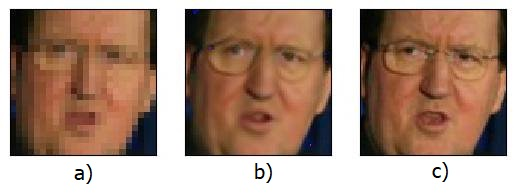
\includegraphics[scale=0.8]{SRGAN.jpg}
\caption{a) fotografija niske rezolucije, b) generirana fotografija visoke rezolucije, c) izvorna fotografija visoke rezolucije \cite{slika1}}
\end{figure}

\subsubsection{CycleGAN}
Postoji mnogo pejzaža koje su naslikali primjerice van Gogh ili Monet, ali za nijedan pejzaž nemamo usporednu fotografiju stvarnog krajolika. CycleGAN izvodi translaciju fotografije, odnosno translatira fotografiju iz jedne domene (npr. krajolik), u drugu domenu (npr. isti pejzaž oslikan stilom van Gogha) u odsutnosti primjera za treniranje. \cite{Tipovi}

\begin{figure}[h]
\centering
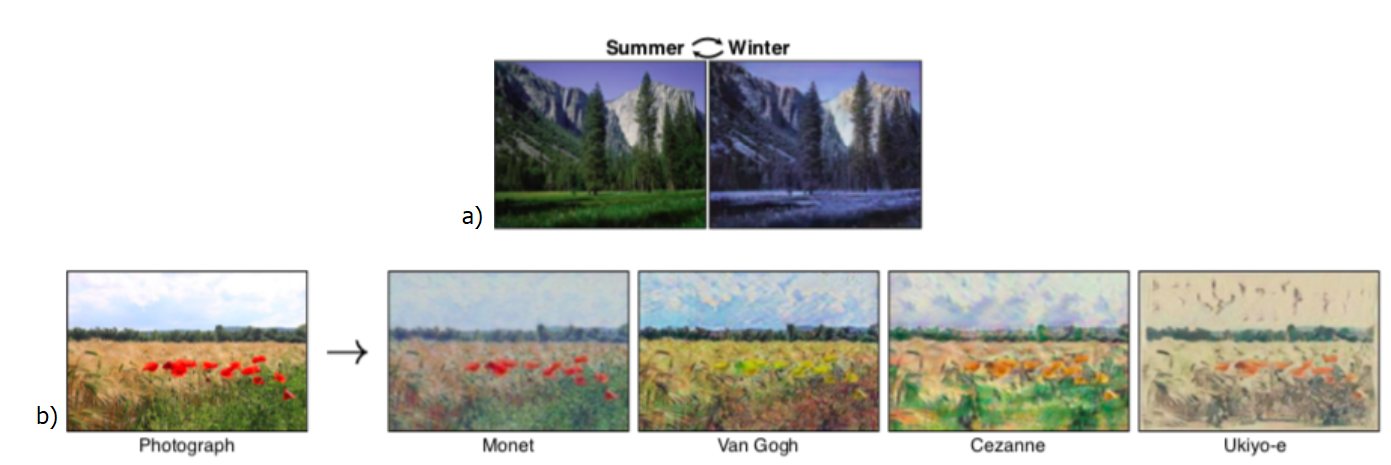
\includegraphics[scale=0.5]{CycleGAN.png}
\caption{a) translacija između dva razdoblja, b) translacija u stilove različitih slikara \cite{Tipovi}}
\end{figure}

\subsubsection{InfoGAN}
InfoGAN nam daje kontrolu nad nekim značajkama generiranih slika. Koristi koncepte iz teorije informacija, kao primjerice na MNIST datasetu upravljanje širinom ili rotacijom znamenki. \cite{Tipovi}

\begin{figure}[h]
\centering
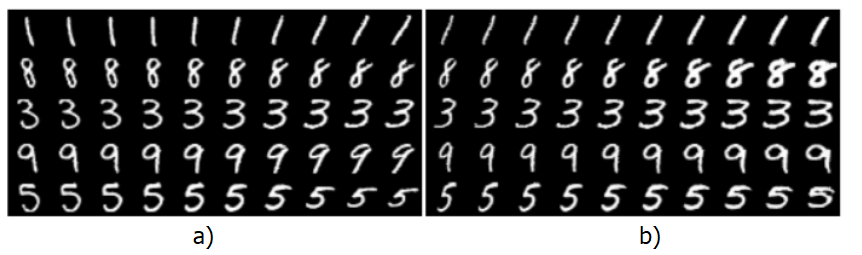
\includegraphics[scale=0.7]{InfoGAN.png}
\caption{a) rotacija znamenaka, b) povećanje širine znamenaka \cite{Tipovi}}
\end{figure}

\subsubsection{StyleGAN}
StyleGAN je tip GAN-a koji može generirati fotografije vrlo visoke rezolucije, čak do 1024x1024 piksela. Ideja je izgraditi hrpu slojeva gdje početni slojevi mogu generirati fotografije niske rezolucije (počevši od 2x2), a daljnji slojevi postepeno povećavaju rezoluciju. Svako otvaranje poveznice https://thispersondoesnotexist.com/, generirat će novo ljudsko lice koje ne postoji. \cite{Style}

\begin{figure}[h]
\centering
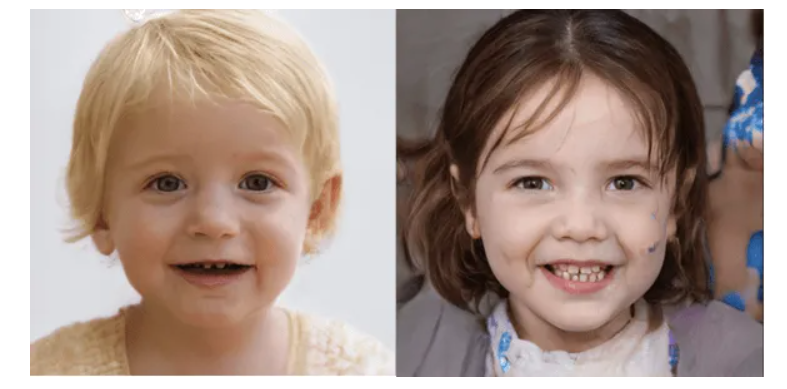
\includegraphics[scale=0.7]{StyleGAN.png}
\caption{Primjeri lica generiranih StyleGAN-om \cite{Style}} 
\end{figure}

\newpage
\section{Primjene GAN-ova}

\begin{figure}[h]
\centering
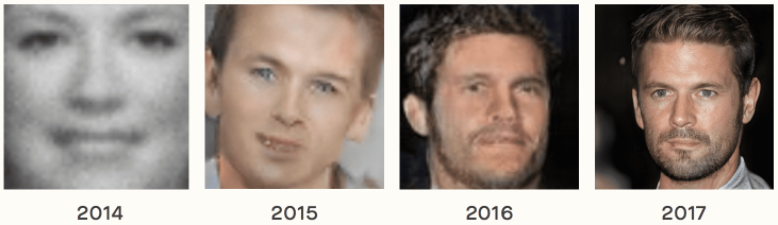
\includegraphics[scale=0.8]{Primjena.png}
\caption{Brzi napredak GAN-ova od 2014. do 2017. godine \cite{slika2}}
\end{figure}

GAN-ovi imaju vrlo specifične, ali zanimljive primjene. Neke od najkorisnijih primjena u današnjem digitalnom svijetu su generiranje fotografija ljudskih lica, generiranje likova iz crtića, generiranje emojija na temelju fotografija stvarnih osoba, uređivanje fotografija, predviđanje videa te generiranje 3D objekata. \cite{slika2}

\begin{figure}[h]
\centering
\includegraphics[scale=0.58]{Crtić.png}
\caption{Generirani crtani likovi \cite{slika2}}
\end{figure}

\begin{figure}[h]
\centering
\includegraphics[scale=0.58]{Kiša.png}
\caption{Brisanje kiše iz fotografija \cite{slika2}}
\end{figure}

\begin{figure}[h]
\centering
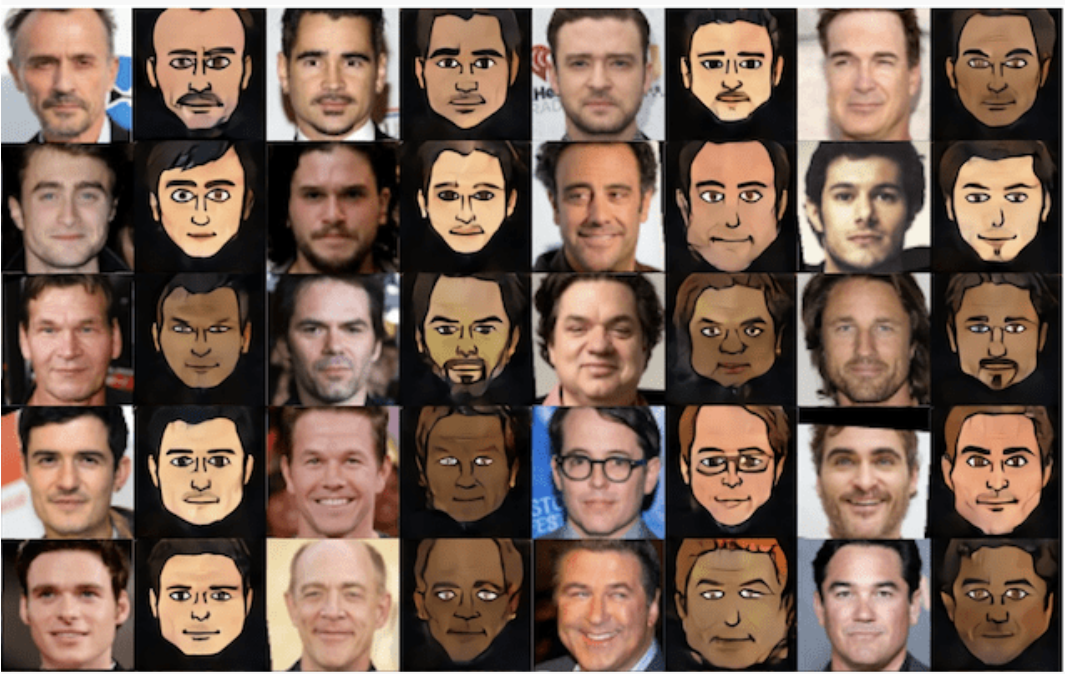
\includegraphics[scale=0.58]{Emoji.png}
\caption{Generirani emojiji na temelju fotografija poznatih osoba \cite{slika2}}
\end{figure}

\begin{figure}[h]
\centering
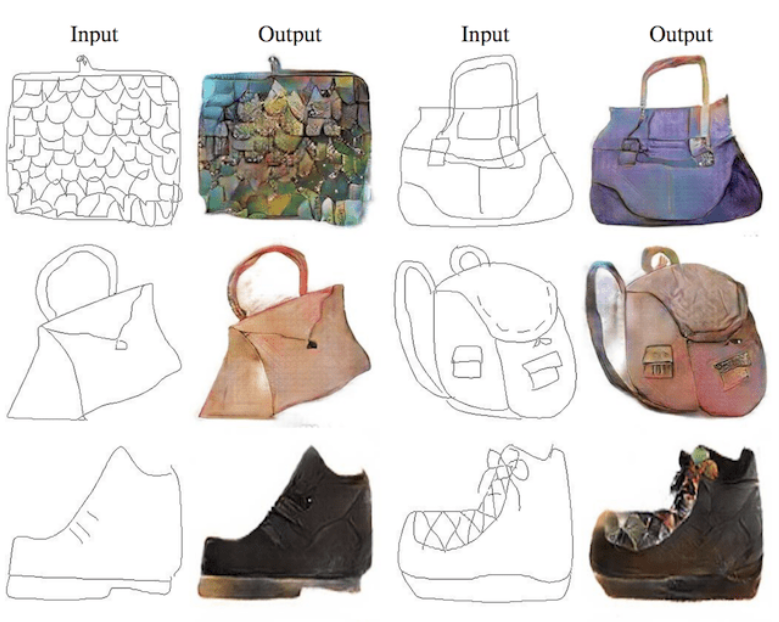
\includegraphics[scale=0.58]{Bojanje.png}
\caption{Bojanje skica \cite{slika2}}
\end{figure}

\chapter{3DGAN}
\section{Uvod i operacije 3D konvolucija}
3DGAN je GAN arhitektura za generiranje 3D objekata. Generiranje 3D objekata je općenito vrlo kompleksno, a 3DGAN je rješenje koje može generirati realistične i raznovrsne 3D oblike. Slično kao obični GAN, 3DGAN ima generator i diskriminator. Obje mreže koriste 3D konvolucijske slojeve, umjesto 2D konvolucija. Ako mu je pruženo dovoljno veliko polje podataka, može naučiti generirati 3D oblike dobre vizualne kvalitete. \cite{3dgan1}

Ukratko, operacije 3D konvolucija primjenjuju 3D filtar na ulazni skup podataka u tri smjera - x, y i z. Ovaj postupak stvara hrpu 3D mape značajki\footnote{Engl. 3D feature maps}. Oblik izlaza sličan je obliku kocke ili kvadra. Slika 4.1 prikazuje postupak 3D konvolucija. Naglašeni dio lijeve kocke je ulazni podatak. U sredini je jezgra\footnote{Engl. kernel}, oblika (3, 3, 3). Desni blok je izlaz postupka konvolucija. \cite{3dgan1}

\begin{figure}[h]
\centering
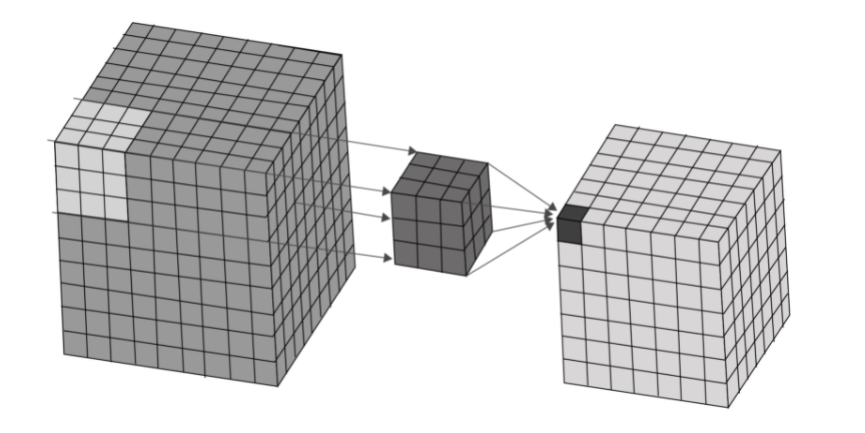
\includegraphics[scale=0.75]{Kocka.png}
\caption{Postupak 3D konvolucije \cite{3dgan1}}
\end{figure}

\newpage

\section{Arhitektura}
Arhitektura 3DGAN-a je potpuno konvolucijska, odnosno svi slojevi u generatoru i diskriminatoru su 3D konvolucijski slojevi i time se 3DGAN nastavlja na DCGAN arhitekturu. S obzirom na to da su im arhitekture simetrične, mreže su međusobno zrcalne jedna drugoj. \cite{3dgan}

Generator \(G\) preslikava latentni vektor \(z\) u željeni trodimenzionalni objekt \(G(z)\). Diskriminator \(D\) daje vrijednost \(D(x)\) koja predstavlja odluku mreže da li je objekt \(x\) stvaran ili umjetno generiran.
Kao i u originalnom Generative Adversarial Networks radu \cite{GAN} koristi se pogreška unakrsne binarne entropije za diskriminator, s L1 normom kao gubitkom generatora, pa je ukupna funkcija gubitka koja se optimizira: \cite{3dgan}

\begin{equation}\label{eq:pythagoras}
 L_{3D-GAN} = log D(x) + log (1 - D(G(z))))
\end{equation}

Slike 4.2 i 4.3 prikazuju konceptualno kako su mreže organizirane, a o detaljima implementacije je više objašnjeno u odjeljku 5.3.

\begin{figure}[h]
\centering
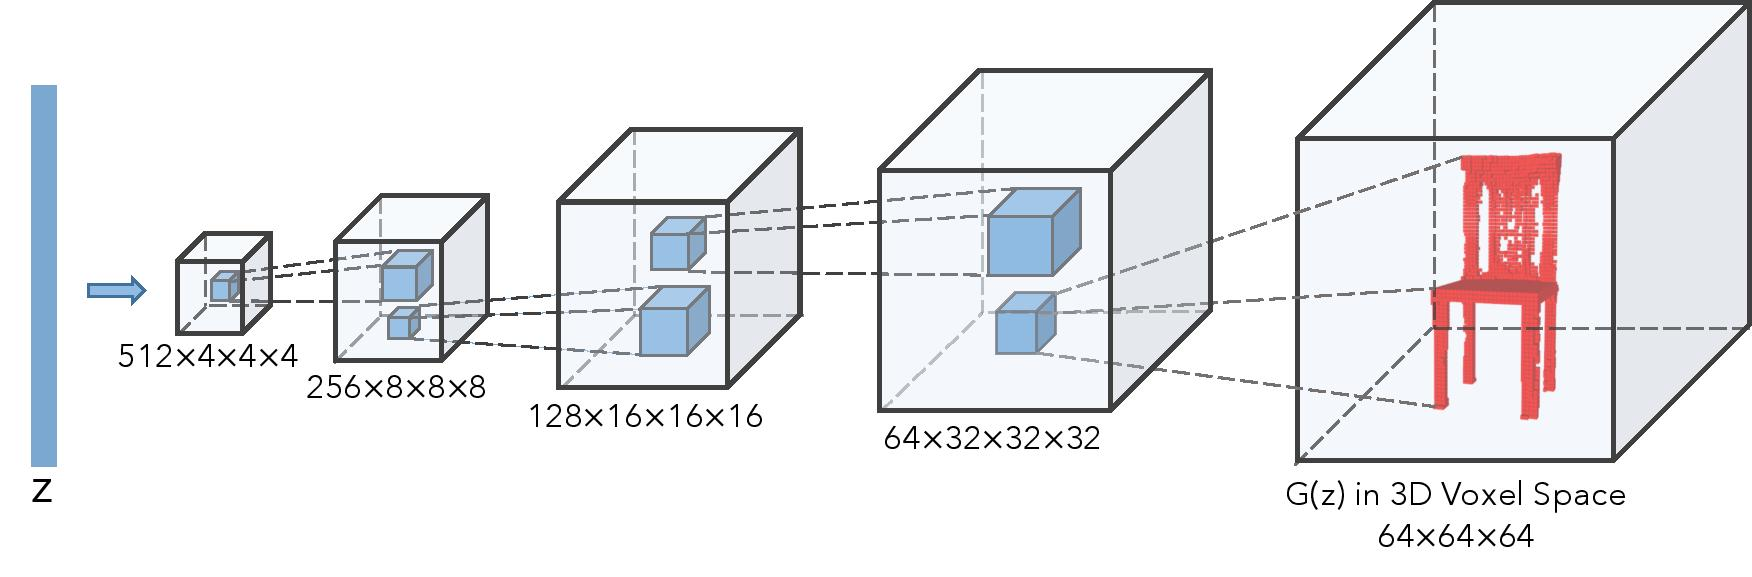
\includegraphics[scale=0.5]{3dgan_gen.jpg}
\caption{Generator 3DGAN-a \cite{3dgan_home}}
\end{figure}

\begin{figure}[h]
\centering
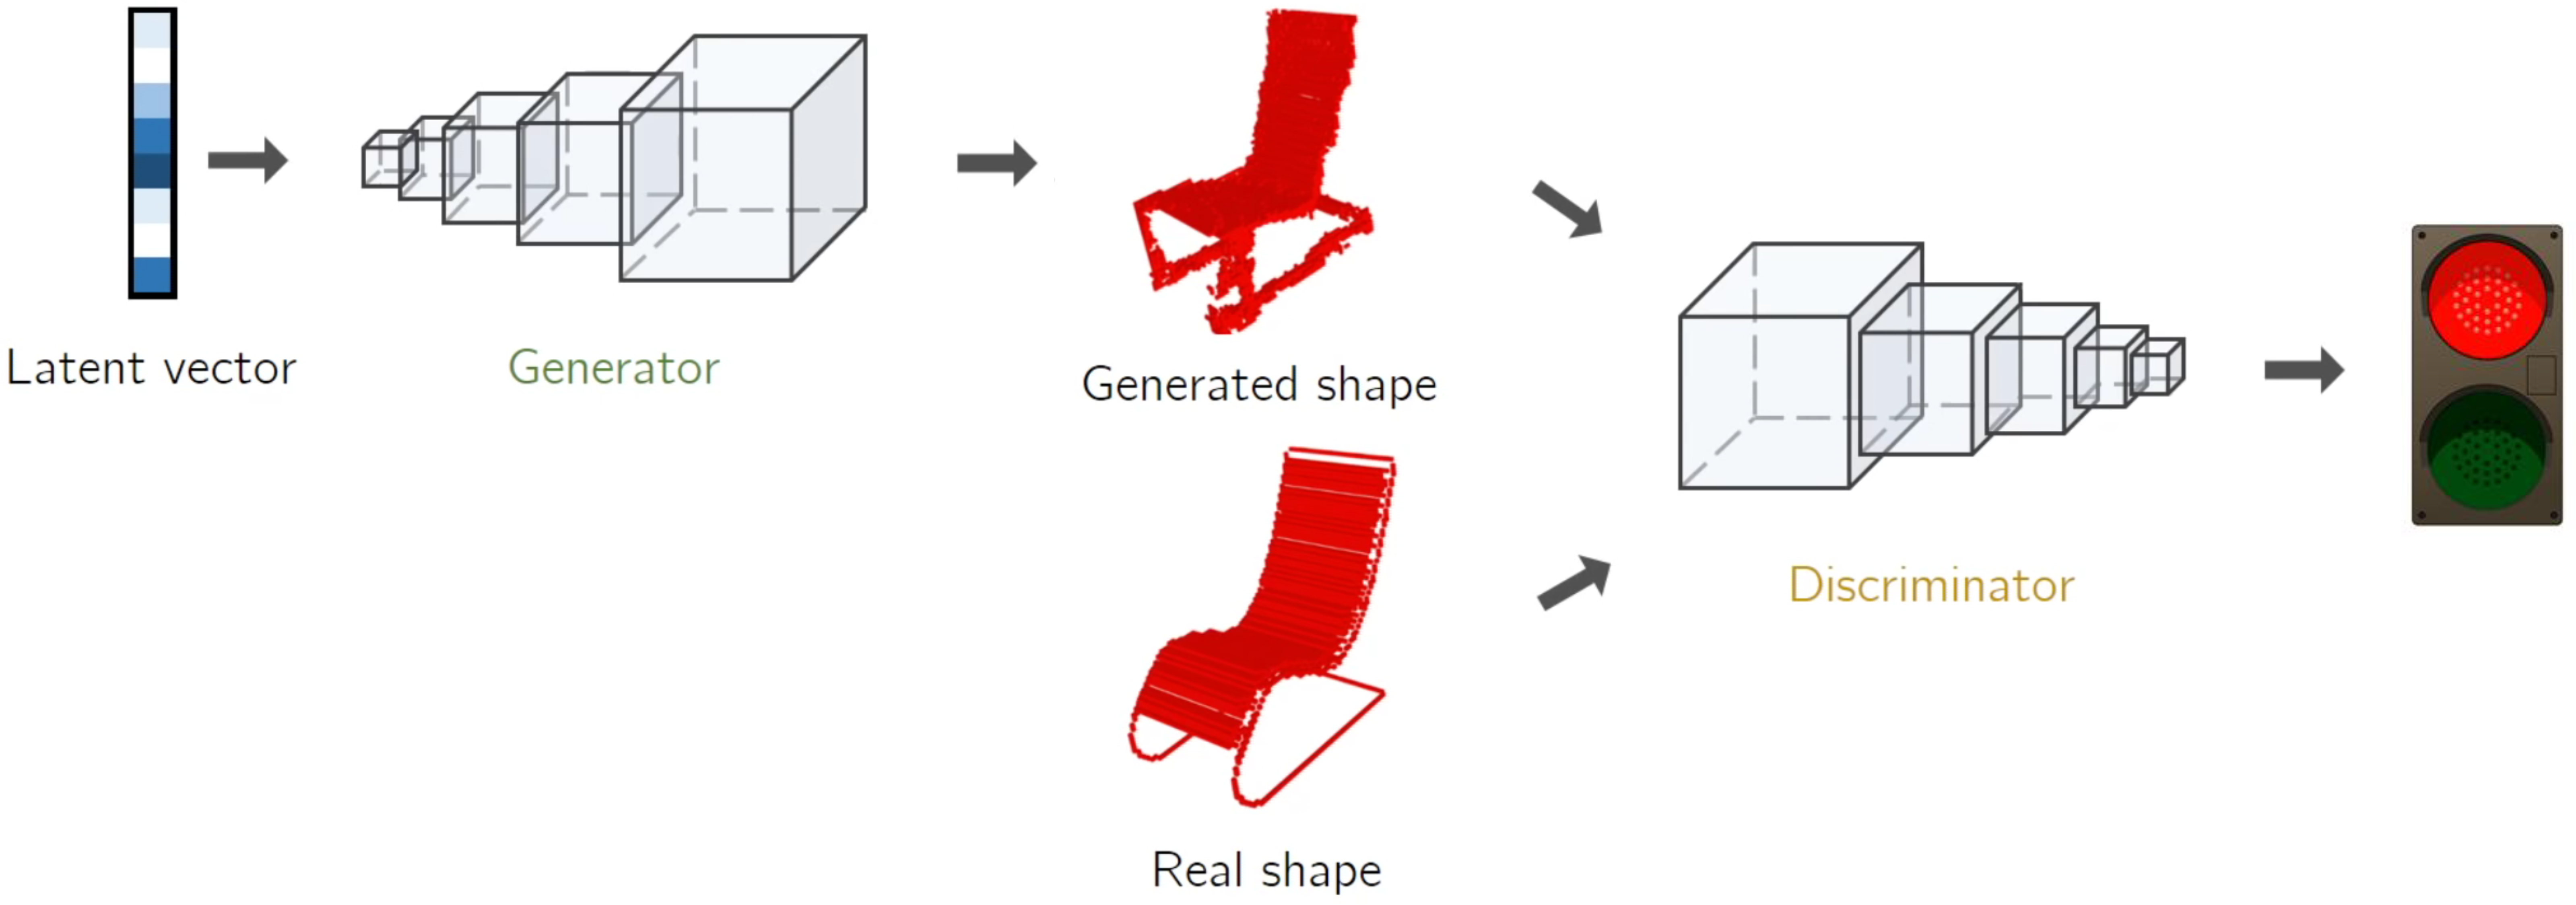
\includegraphics[scale=0.25]{3DGAN_all.png}
\caption{3DGAN sustav \cite{3dgan_all}}
\end{figure}

\break

\chapter{Implementacija i primjenjene tehnologije}
Ideja ovog rada je razviti sustav za duboko učenje; treniranje 3DGAN mreže, generiranje 3D modela, njihova vizualizacija uz usporedbu sa stvarnim modelima te generiranje ultrazvučnih slika defekata u materijalu. Implementacija je ostvarena u programskom jeziku Python, koristeći biblioteke PyTorch, matplotlib, scikit, NumPy i Visdom. Model neuronske mreže se trenirao na sustavu Google Colab u Jupyter bilježnici, dok je kod uređivan u Visual Studio Code integriranom okruženju.

\subsubsection{Python}
Python je dinamički pisan generalni programski jezik visoke razine. S obzirom na to da mu se kod automatski kompilira u bajt kod te izvršava, Python je prikladan kao skriptni jezik za implementacije kraćih programa te Web aplikacija. Dosljedna korištenost objektno-orijentirane paradigme i naglašavanje čitljivosti koda čine Python jednostavnim za korištenje, a velika zbirka biblioteka, od kojih su mnoge pisane u C-u, s mogućnošću korištenja C i C++ koda, također ga čini korisnim i za računalno intenzivne zadaće. \cite{Python} Jedan je od najkorištenijih jezika u područjima strojnog učenja i obrade podataka s podržanim bibliotekama za strojno učenje TensorFlow i PyTorch.

\subsubsection{PyTorch}
PyTorch je optimizirana biblioteka za strojno učenje temeljena na Torch biblioteci. Razvijena od strane Facebook-ovog laboratorija za istraživanje umjetne inteligencije FAIR, besplatna je za korištenje te je otvorenog koda. Originalno implementirana u C-u te Lua skriptnom jeziku, PyTorch omogućava rad u Pythonu te nudi visoku razinu GPU optimizacije. Najveći dio čine biblioteke za manipulaciju tenzorima i rad s neuronskim mrežama te alati za treniranje mreža. Može se koristiti s bibliotekama poput NumPy, SciPy i Cython. \cite{Pytorch_article}

\subsubsection{NumPy}
NumPy je jedan od osnovnih paketa za znanstvene proračune u Python-u. Ova biblioteka definira objekt multidimenzionalnog niza, objekte izvedene iz njega te velik izbor funkcija za brze operacije nad njima, poput logičkih, sortiranje, selekcija, Fourier-ove transformacije, linearna algebra, statističke operacije i još mnogo toga.
Objekt \textit{ndarray} obuhvaća n-dimenzionalne nizove homogenih podatkovnih tipova, dok se mnoge operacije izvršavaju u kompiliranom kodu u svrhu poboljšanja performansi. Osnovne razlike između NumPy niza i običnih Python nizova su:
\begin{itemize}
    \item \textit{ndarray} ima fiksne dimenzije kod kreiranja, dok se Python nizovi mogu povećavati dinamički
    \item svi elementi \textit{ndarray-a} moraju biti istog podatkovnog tipa kako bi bili iste veličine u memoriji
    \item NumPy nizovi olakšavaju napredne matematičke i druge operacije na velikoj količini podataka
    \item sve veća količina znanstvenih i matematičkih Python biblioteka koristi NumPy nizove
    \cite{numpy}
\end{itemize}

\subsubsection{Matplotlib}
Matplotlib je biblioteka za grafički prikaz podataka, originalno napravljena za emuliranje grafičke naredbe MATLAB-a. Dizajnirana je kako bi što više pojednostavila kreiranje jednostavnih grafova, ponekad u samo jednoj naredbi. Konceptualno se razdvaja na tri djela:
\begin{itemize}
    \item \textit{pylab} sučelje je skup funkcija koje omogućavaju korisniku kreiranje grafova s kodom sličnim MATLAB-ovom
    \item \textit{Matplotlib API} je skup klasa koje rade računski teške zadaće, kreiranje i raspolaganje figurama, tekstom, linijama i slično
    \item \textit{backend}, odnosno pozadinska aplikacija, skup je uređaja za prikaz koji transformiraju \textit{frontend} zapis u izlazni oblik
    \cite{matplotlib}
\end{itemize}

\break

\section{Organizacija programskog koda}
Sav programski kod je pisan u jeziku Python verzije 3.6.9. Organiziran je u jednom direktoriju, u nekoliko datoteka:
\begin{itemize}
    \item \textbf{main.py} - skripta pokretač programa, prikuplja programske argumente te navigira treniranje odnosno testiranje neuronske mreže
    \item \textbf{model.py} - definicija modela neuronske mreže, prema 3DGAN modelu
    \item \textbf{train.py} - kod zadužen za učenje težina mreže te pohranu i dohvaćanje kontrolnih točaka
    \item \textbf{test.py} - pokretanje modela iz kontrolnih točaka te generiranje objekata
    \item \textbf{visualize.py} - vizualizacija objekata pomoću Visdom alata ili matplotlib biblioteke
    \item \textbf{visualize\_2D.py} - skripta za dohvaćanje modela i automatsko generiranja ultrazvučnih dvodimenzionalnih slika pukotina
    \item \textbf{dataset\_utils.py} - skripta za manipulaciju ulaznim podatcima
    \item \textbf{params.py} - globalni parametri za treniranje mreže te rad s podatcima
\end{itemize}

U nastavku su izdvojene najvažnije komponente te je dan njihov programski kod.

\section{Podaci za treniranje}
Inicijalno učenje mreže za generiranje 3D modela objekata rađeno je s ModelNet40 \cite{modelNet} skupom podataka. Princeton ModelNet sakupljen je da omogući istraživačima u područjima računalnog vida, grafike i robotike rad s urednom kolekcijom 3D CAD objekata. Kako bi izabrali kategorije objekata, znanstvenici s Princetona sastavili su listu najčešćih kategorija objekata na svijetu, koristeći statistiku iz SUN baze podataka. Modeli se nalaze u 40 kategorija, te postoji i prebran skup od 10 kategorija. \cite{modelNet} Modeli su iz originalnog Object File Format-a (.off),  koji specificira poligone na površini modela,  prevedeni u trodimenzionalne nizove te pohranjeni u MATLAB (.mat) datoteke. Trodimenzionalni nizovi predstavljaju popis voksela, gdje jedinica znači da voksel postoji, a nula označava prazan prostor. Modeli za treniranje skalirani su u kocke dimenzija 32x32x32, odnosno 64x64x64 voksela.

Drugi dio rada, generiranje slika pukotina u materijalu, rađen je nad skupom podataka veličine 128x128x128. Podaci su skalirani u raspon \([0, 1]\).

\section{Model i treniranje}
Model mreže rađen je u skladu s PyTorch bibliotekom za oblikovanje neuronskih mreža. Za učenje i generiranje modela ultrazvučnih slika, zbog veće dimenzionalnosti modela dodan je po jedan 3D konvolucijski sloj u generator i diskriminator, te je ovdje opisana ta mreža.

\textbf{Diskriminator} se sastoji od 6 3D konvolucijskih slojeva. On kao ulaz prima seriju od 8 objekta dimenzija 128x128x128, te se u svakom sljedećem sloju dimenzije smanjuje za faktor 2 do izlaznog sloja kojemu je izlaz tenzor veličine 8x1, po jedna vrijednost za svaki objekt na ulazu, iz raspona \([0, 1]\).  

\textbf{Generator} se sastoji od 6 potpuno konvolucijskih slojeva koji vrše transponiranu konvoluciju. Na ulaz mu postavljamo 200-dimenzionalni vektor koji se za svaki prolaz mreže generira iz Gaussove raspodjele, kako bi se unijela nasumičnost u generativna svojstva mreže.

Između svih slojeva također se nalazi sloj za normalizaciju serije\footnote{engl. batch normalization layer}, koji standardizira ulaze u sloj za svaku seriju pomoću centriranja i skaliranja. Diskriminator između slojeva ima LeakyReLU aktivacijsku funkciju, dok generator ima ReLU\footnote{engl. Rectified Linear Unit} (Slika 5.1). Obje mreže na izlaznom sloju imaju sigmoidalnu aktivacijsku funkciju. Veličine jezgri su 4, a za pomak\footnote{engl. stride} se uzima 2.

\begin{figure}[h]
\centering
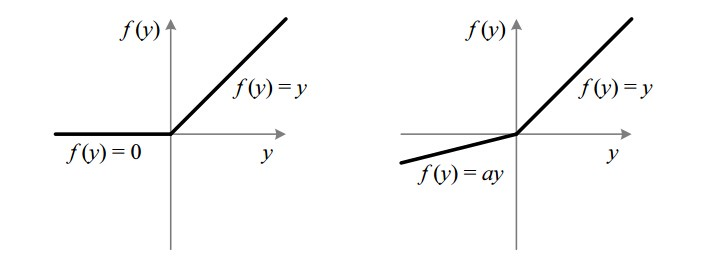
\includegraphics[scale=0.58]{relu-vs-leaky.jpeg}
\caption{Usporedba ReLU (lijevo) i LeakyReLU aktivacijskih funkcija \cite{ReLU}}
\end{figure}

U nastavku, isječak 5.1 i isječak 5.2 prikazuju specifikaciju obje mreže.

\break

\begin{lstlisting}[language=Python, caption=Modificirani 3DGAN model diskriminatora]
class net_D(torch.nn.Module):
    def __init__(self, args):
        (...)

        self.f_dim = 32
        self.layer1 = self.conv_layer(1, self.f_dim, kernel_size=4, stride=2, padding=(1,1,1), bias=self.bias)
        self.layer2 = self.conv_layer(self.f_dim, self.f_dim*2, kernel_size=4, stride=2, padding=(1,1,1), bias=self.bias)
        self.layer3 = self.conv_layer(self.f_dim*2, self.f_dim*4, kernel_size=4, stride=2, padding=(1,1,1), bias=self.bias)
        self.layer4 = self.conv_layer(self.f_dim*4, self.f_dim*8, kernel_size=4, stride=2, padding=(1,1,1), bias=self.bias)

        self.layer5 = torch.nn.Sequential(
            torch.nn.Conv3d(self.f_dim*8, 1, kernel_size=4, stride=2, bias=self.bias, padding=padd),
            torch.nn.Sigmoid()
        )

    def conv_layer(self, input_dim, output_dim, kernel_size=4, stride=2, padding=(1,1,1), bias=False):
        layer = torch.nn.Sequential(
            torch.nn.Conv3d(input_dim, output_dim, kernel_size=kernel_size, stride=stride, bias=bias, padding=padding),
            torch.nn.BatchNorm3d(output_dim),
            torch.nn.LeakyReLU(self.leak_value, inplace=True)
        )
        return layer

    def forward(self, x):
        out = x.view(-1, 1, self.cube_len, self.cube_len, self.cube_len)
        out = self.layer1(out)
        out = self.layer2(out)
        out = self.layer3(out)
        out = self.laer4(out)
        out = self.layer5(out)
        out = torch.squeeze(out)
        return out

\end{lstlisting}

\break

\begin{lstlisting}[language=Python, caption=Modificirani 3DGAN model generatora]
class net_G(torch.nn.Module):
    def __init__(self, args):
        (...)

        self.layer1 = self.conv_layer(self.z_dim, self.f_dim*8, kernel_size=4, stride=2, padding=padd, bias=self.bias)
        self.layer2 = self.conv_layer(self.f_dim*8, self.f_dim*4, kernel_size=4, stride=2, padding=(1, 1, 1), bias=self.bias)
        self.layer3 = self.conv_layer(self.f_dim*4, self.f_dim*2, kernel_size=4, stride=2, padding=(1, 1, 1), bias=self.bias)
        self.layer4 = self.conv_layer(self.f_dim*2, self.f_dim, kernel_size=4, stride=2, padding=(1, 1, 1), bias=self.bias)
        
        self.layer5 = torch.nn.Sequential(
            torch.nn.ConvTranspose3d(self.f_dim, 1, kernel_size=4, stride=2, bias=self.bias, padding=(1, 1, 1)),
            torch.nn.Sigmoid()
        )

    def conv_layer(self, input_dim, output_dim, kernel_size=4, stride=2, padding=(1,1,1), bias=False):
        layer = torch.nn.Sequential(
            torch.nn.ConvTranspose3d(input_dim, output_dim, kernel_size=kernel_size, stride=stride, bias=bias, padding=padding),
            torch.nn.BatchNorm3d(output_dim),
            torch.nn.ReLU(True)
        )
        return layer

    def forward(self, x):
        out = x.view(-1, self.z_dim, 1, 1, 1)
        out = self.layer1(out)
        out = self.layer2(out)
        out = self.layer3(out)
        out = self.layer4(out)
        out = self.layer5(out)
        out = torch.squeeze(out)
        return out

\end{lstlisting}

\subsubsection{Treniranje}
U prošlosti, razvoj dubokog učenja ograničavali su slabiji računalni resursi, dok se danas mogu koristiti sve veći i složeniji modeli. No i uz optimizacije biblioteka poput PyTorcha i izvršavanje koda na grafičkoj kartici, proces učenja mreže može trajati tjednima. U tu svrhu često se koriste vanjski servisi poput Google Colaboratory-ja. Colab je servis za izvršavanje Python koda iz preglednika, korištenjem besplatnih grafičkih kartica i Google-ovih vlastitih \textit{Tensor Processing Unit-a (TPU)}, besplatno, u obliku Jupyter bilježnica. Uz profesionalne grafičke kartice, dostupno je 12 GB radne memorije i preko 200 GB prostora na disku. Radno okruženje na Colab-u uključuje dostupne biblioteke za rad s podacima u Python-u -  TensorFlow, Numpy, Matplotlib, Scikit-learn i mnoge druge, a mogu se i učitati dodatne biblioteke poput PyTorch po potrebi.

PyTorch i TensorFlow imaju vlastite rutine za upravljanje skupovima podataka i kolekciju najpopularnijih skupova dostupnih za učitavanje. U ovom radu korištena je mogućnost povezivanja Google-ovog servisa s njihovom vlastitom uslugom udaljene pohrane podataka, Google Drive, kako bi se kod mogao organizirati u datoteke i koristiti vlastite skupove podataka za učenje. 

\begin{figure}[h]
\centering
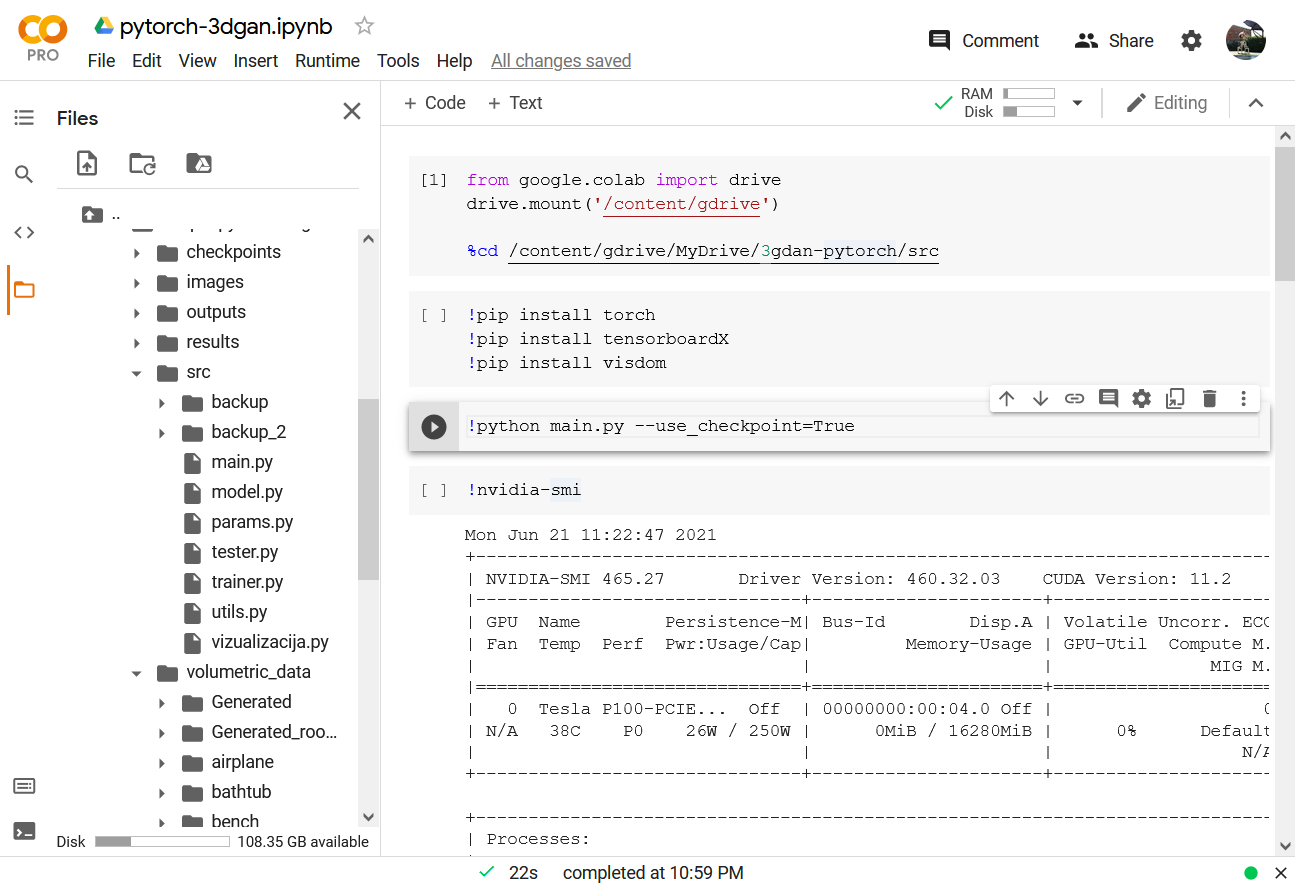
\includegraphics[scale=0.42]{colab_interface.png}
\caption{Sučelje usluge Google Colaboratory}
\end{figure}

Postupak učenja započinje učitavanjem podataka i, po potrebi, modela iz prethodne kontrolne točke. Korišteni parametri definirani su u datoteci \textit{params.py} i za prvotno učenje nad skupom ModelNet40 oni su sljedeći:
\begin{itemize}
    \item broj epoha: 500
    \item broj primjera u seriji: 32
    \item dimenzija vektora šuma Z: 200
    \item broj koraka nakon koliko se sprema model: 10
    \item stopa učenja diskriminatora: 0.00001
    \item stopa učenja generatora: 0.0025
    \item koeficijent LeakyReLU sloja: 0.2
    \item dimenzija kocke voksela: 64
\end{itemize}

U datoteci \textit{train.py} definirane su funkcije gubitka i postupci optimizacije korišteni za učenje. Korištena funkcija gubitka prati specifikaciju u 3DGAN radu, pa se za diskriminator koristi binarna unakrsna entropija, a za generator L1 gubitak, koji su definirani u paketu \textit{torch.nn.BCELoss} odnosno \textit{torch.nn.L1Loss}. Postupak optimizacije je Adam, jedan od najčešće korištenih i najboljih algoritama optimizacije funkcije gubitka, definiran u \textit{torch.optim.Adam}. Na slici 5.3. a) vidimo promjenu gubitka diskriminatora za stvarne modele gitara, a na slici 5.3 b) vidimo isto za generirane modele.

\begin{figure}[H]
\centering
\begin{subfigure}[b]{0.8\textwidth}
   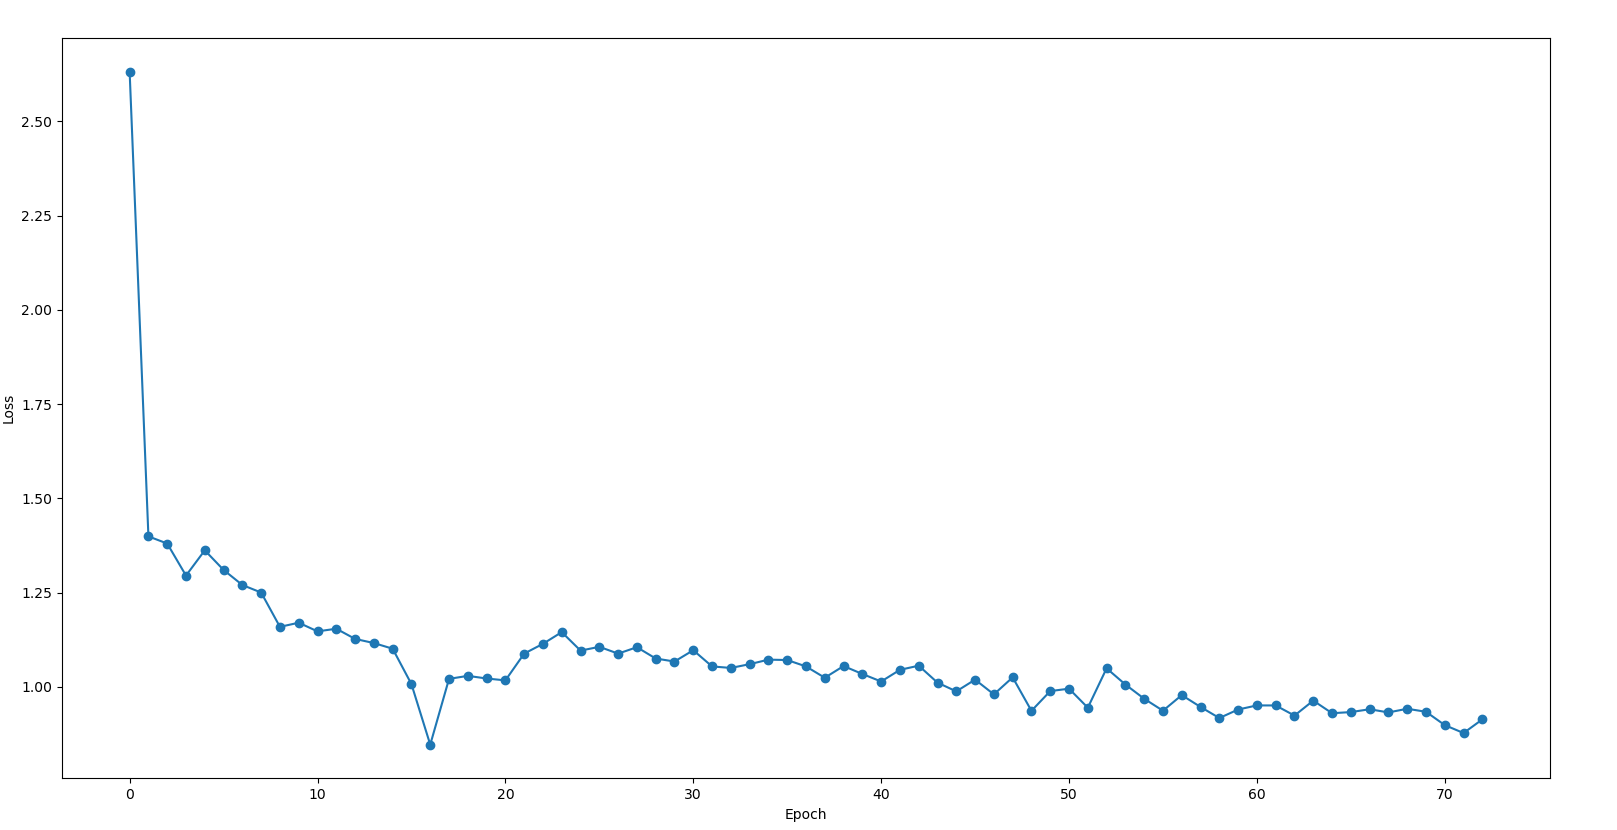
\includegraphics[width=1\linewidth]{D(x).png}
   \label{fig:Ng1} 
    \caption{D(x)}
\end{subfigure}

\begin{subfigure}[b]{0.8\textwidth}
   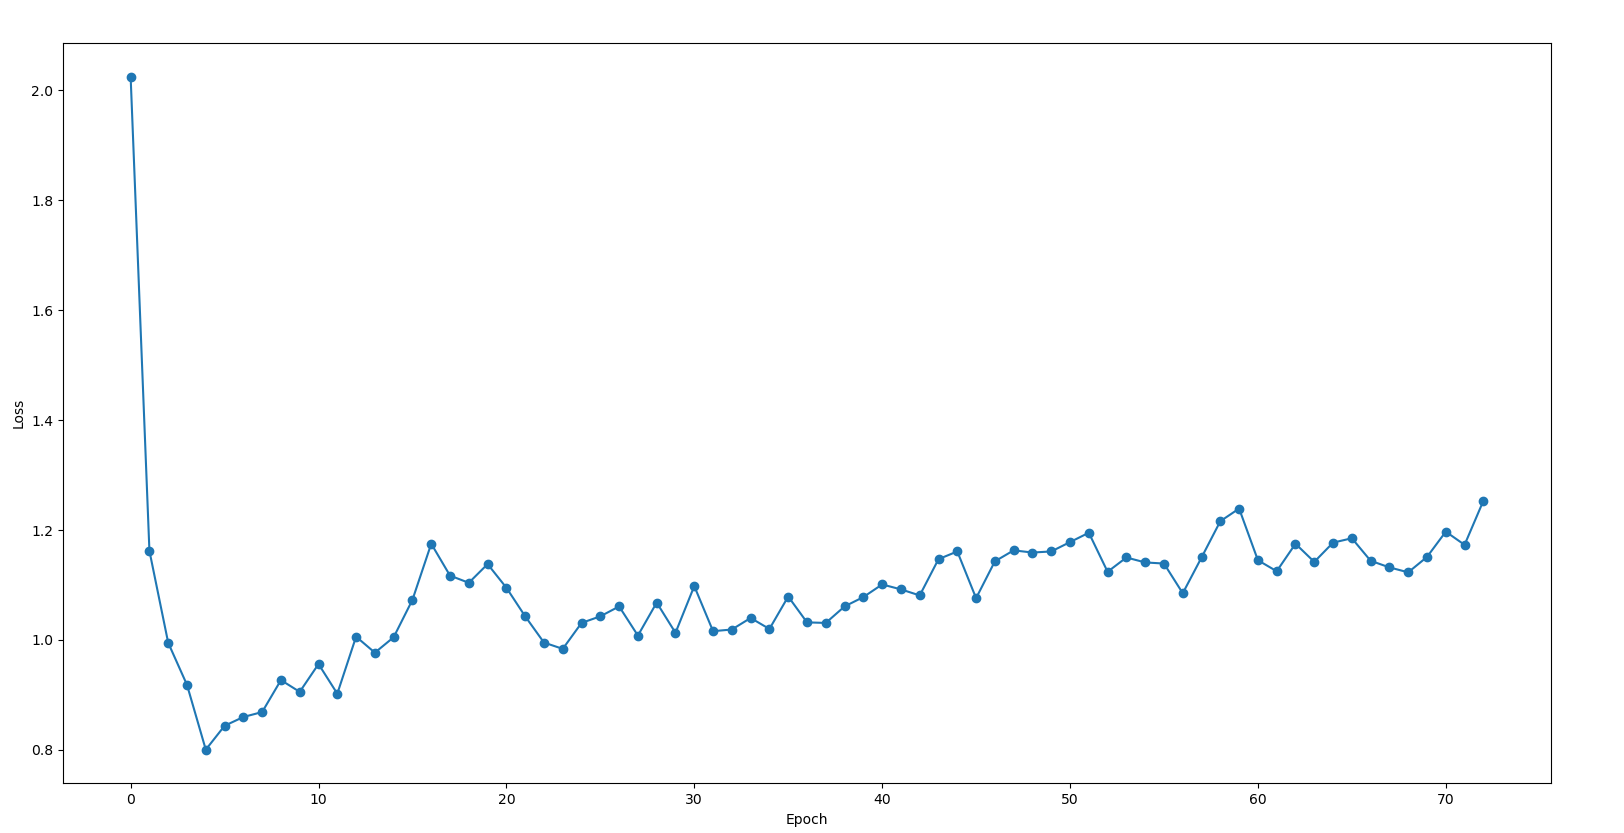
\includegraphics[width=1\linewidth]{D(G(x)).png}
   \label{fig:Ng2}
   \caption{D(G(x))}
\end{subfigure}
\caption{Funkcija gubitka kroz epohe}
\end{figure}

\break

U ranijim fazama učenja boljim su se pokazale vrijednosti stope učenja od 0.0025 za generator i 0.00001 za diskriminator, od predloženih 0.001 za generator i 0.00005 za diskriminator. U većini slučajeva, pogotovo u skupovima objekata s manjim brojem primjera, za učenje je bilo dovoljno 200 epoha, dok je u nekim slučajevima učenje napredovalo i nakon 500. epohe. Broj primjera koji se uzima u serije ovisi o memoriji dostupnoj na grafičkoj kartici. Za učenje ModelNet40 objekata korištena je veličina serije 32, dok je za učenje nad većim, ultrazvučnim slikama pukotina u materijalu,  korištena veličina serije 8. Povećanje dimenzija ulaznog vektora šuma u generator pokazalo je utjecaj na složenost i raznolikost generiranih primjera. Povećanje dimenzionalnosti s 32x32x32 na 64x64x64 uvelike usporava učenje, kako veličina primjera raste 8 puta s dvostrukim povećanjem stranice kocke, ali također daje mnogo kvalitetnije primjere, čak i nad istim skupom podataka samo skaliranim na veće dimenzije.

\subsubsection{Učitavanje i spremanje modela}

PyTorch omogućuje spremanje i učitavanje težina i drugih značajki mreže, što je nužnost i dobra praksa kod dugih izvođenja programa. Google Colab u pokušaju da svima omogući korištenje besplatnih resursa provodi optimizaciju dostupnosti okruženja te ograničava korištenje sustava na 12 sati rada odjednom, što učitavanje pospremljenih modela čini korisnim za nastavak izvođenja programa. Isječak 5.3 i isječak 5.4 prikazuju jednostavnost implementacije ovih postupaka pomoću PyTorch funkcija \textit{torch.load} i \textit{torch.save}. Za korištenje modela za inferenciju, odnosno generiranje primjera nakon treniranja dovoljno je pohraniti modele, dok je za nastavak treniranja potrebno sačuvati i rječnik stanja optimizatora i funkcije gubitka.


\begin{lstlisting}[language=Python, caption=Kod za spremanje kontrolnih točaka]
if (epoch + 1) % params.model_save_step == 0:

    torch.save(G.state_dict(), params.output_dir + '/' + args.model_name + '/' + 'G_' + str(epoch) + '.pth')
    torch.save(D.state_dict(), params.output_dir + '/' + args.model_name + '/' + 'D_' + str(epoch) + '.pth')

    torch.save({
        'epoch': epoch,
        'G_optimizer_state_dict': G_solver.state_dict(),
        'D_optimizer_state_dict': D_solver.state_dict(),
        'loss_G': criterion_G,
        'loss_D': criterion_D
    }, params.checkpoint_dir + '/checkpoint_' + str(epoch) + '.tar')

\end{lstlisting}

\break

\begin{lstlisting}[language=Python, caption=Kod za učitavanje kontrolnih točaka]
    start_epoch = 0

    if args.use_checkpoint == True:

        for filename in os.listdir(params.checkpoint_dir):
            if filename.startswith("checkpoint_"):
                check_epoch = int(filename[11:-4])
                print("checkpoint epoch: ", check_epoch)
                if check_epoch > start_epoch:
                    start_epoch = check_epoch
                    
        if start_epoch != 0:

            save_file_path = params.output_dir + '/' + args.model_name
            pretrained_file_path_G = save_file_path + '/' + 'G_' + str(start_epoch) + '.pth'
            pretrained_file_path_D = save_file_path + '/' + 'D_' + str(start_epoch) + '.pth'

            if not torch.cuda.is_available():
                G.load_state_dict(torch.load(pretrained_file_path_G, map_location={'cuda:0': 'cpu'}))
                D.load_state_dict(torch.load(pretrained_file_path_D, map_location={'cuda:0': 'cpu'}))
                checkpoint = torch.load(params.checkpoint_dir + '/checkpoint_' + str(start_epoch) + '.tar', map_location={'cuda:0': 'cpu'})
            else:
              G.load_state_dict(torch.load(pretrained_file_path_G))
              D.load_state_dict(torch.load(pretrained_file_path_D))
              D.to(params.device)
              G.to(params.device)
              criterion_D.to(params.device)
              criterion_G.to(params.device)
              print("trazimo: ", params.checkpoint_dir + '/checkpoint_' + str(start_epoch) + '.tar')
              checkpoint = torch.load(params.checkpoint_dir + '/checkpoint_' + str(start_epoch) + '.tar')

            D_solver.load_state_dict(checkpoint['D_optimizer_state_dict'])
            G_solver.load_state_dict(checkpoint['G_optimizer_state_dict'])
            start_epoch = checkpoint['epoch']
            criterion_D = checkpoint['loss_D']
            criterion_G = checkpoint['loss_G']

    else:
        D.to(params.device)
        G.to(params.device)

\end{lstlisting}

\break

\section{Vizualizacija modela}
Kod generativnih modela teško možemo imati klasičnu mjeru uspješnosti modela, poput postotka točno klasificiranih primjera. Pogreške učenja su dobar pokazatelj rada mreže, ali nisu u izravnoj korelaciji sa složenošću i realizmom generiranih modela. Generativna sposobnost mreže je subjektivna i može se pratiti samo vizualiziranjem primjera i njihovom usporedbom sa stvarnim primjerima. U tu svrhu korištena je matplotlib biblioteka za vizualizaciju i pohranu dvodimenzionalnih slika, te Visdom za interaktivnu trodimenzionalnu vizualizaciju.

\textbf{Visdom} je fleksibilan alat za kreiranje, organiziranje i dijeljenje velikih količina podataka uživo i podržava Python. Visdom pruža sučelje za organizaciju grafičkih prikaza kojemu se pristupa preko Web preglednika. \cite{visdom} Vizualizacija grafova se obavlja preko Plotly-jevih biblioteka, a sučelje tog alata je prikazano na slici 5.4.
\\

\begin{figure}[h]
\centering
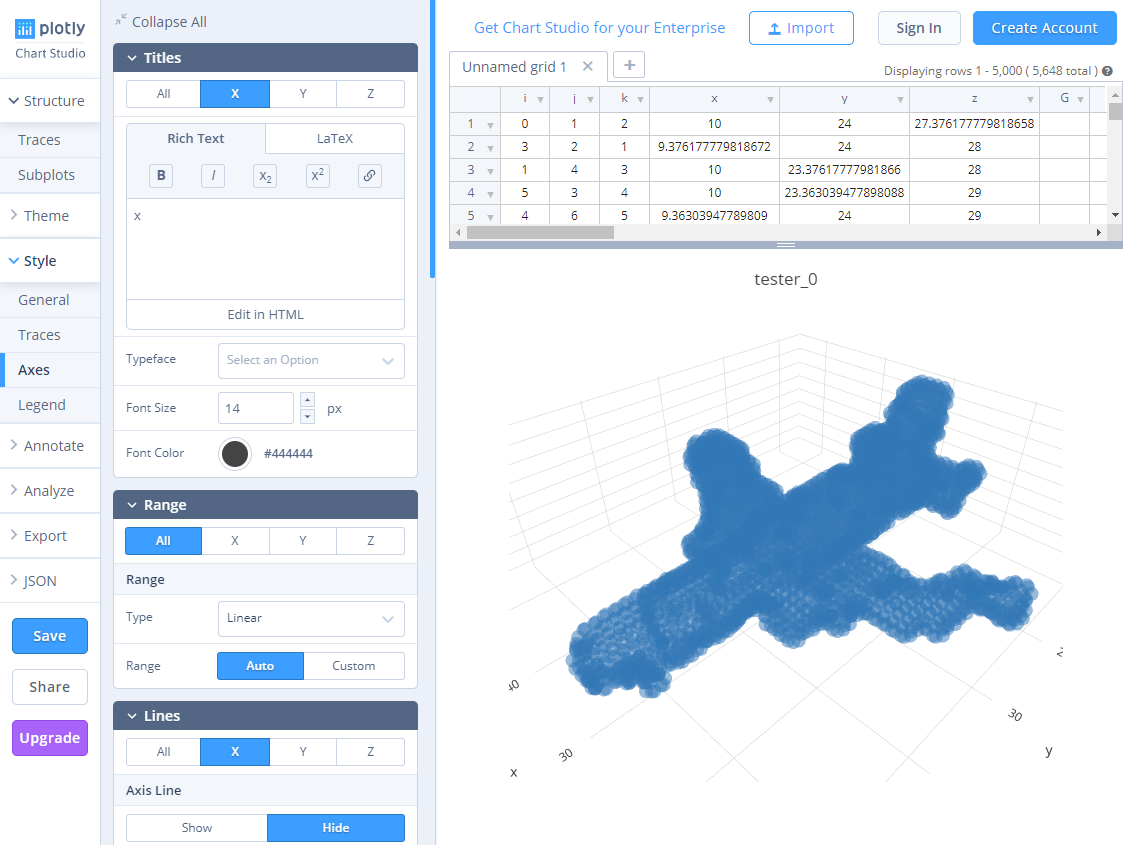
\includegraphics[scale=0.5]{sucelje_plotly.png}   
\caption{Sučelje alata Plotly}
\end{figure}

\break

Isječak 5.5 prikazuje osnovni kod koji učitava pohranjene modele, generira 8 uzoraka te ih prikazuje pomoću Visdom poslužitelja.
\\

\begin{lstlisting}[language=Python, caption=Kod za vizualizaciju pomoću alata Visdom]

def getVFByMarchingCubes(voxels, threshold=0.25):
    v, f = sk.marching_cubes_classic(voxels, level=threshold)
    return v, f


def plotVoxelVisdom(voxels, visdom, title):
    v, f = getVFByMarchingCubes(voxels)
    visdom.mesh(X=v, Y=f, opts=dict(opacity=0.5, title=title))
    
(...)

def testModel(args):
    vis = visdom.Visdom()
    
    save_file_path = params.output_dir + '/' + args.model_name
    pretrained_file_path_G = save_file_path+'/'+'G.pth'
    pretrained_file_path_D = save_file_path+'/'+'D.pth'
    
    D = net_D(args)
    G = net_G(args)
    
    G.load_state_dict(torch.load(pretrained_file_path_G))
    D.load_state_dict(torch.load(pretrained_file_path_D))
    
    G.to(params.device)
    D.to(params.device)
    G.eval()
    D.eval()
    
    N = 8
    
    for i in range(N):
        z = generateZ(args, 1)
    
        fake = G(z)
        
        samples = fake.unsqueeze(dim=0).detach().numpy()
        y_prob = D(fake)
        y_real = torch.ones_like(y_prob)
    
        plotVoxelVisdom(samples[0,:], vis, "tester_"+str(i))
    

\end{lstlisting}

\break

Za vizualizaciju ultrazvučnih pukotina u materijalu dodatno je korištena matplotlib vizualizacija za dvodimenzionalni prikaz pukotina. Napravljena je skripta za prikaz presjeka modela na mjestu gdje je pukotina najveća.\\
Skripta se sastoji od par dijelova:
\begin{enumerate}
    \item učitavanje modela generatora
    \item generiranje skupa primjera
    \item dodavanje krova primjerima
    \item pronalazak koordinate za koju je najveći presjek pukotina
    \item vizualizacija presjeka i pohrana slike
\end{enumerate}

Dodavanje "krova" primjerima odnosi se na materijal od kojeg se odbije ultrazvučna slika, koji se nalazi u istom obliku na svim primjerima, što je vidljivo na rezultatima niže. Krov je prije treniranja obrisan sa svih primjera kako bi mreža učila generirati oblike pukotina, bez potrebe da uči generirati taj volumno velik dio primjera koji je konstantan svima od njih. 

Pronalazak koordinate presjeka za koji je najveća površina pukotine je jednostavan. Prvo odaberemo po kojoj osi tražimo presjek, a kako je okolni prostor pukotinama prazan (uz iznimku krova), vrijednost ostalih voksela je fiksna granična vrijednost, pa se sumiranjem svih voksela u određenom presjeku dobije vrijednost koja se može usporediti s drugim vrijednostima. Konkretno u ovom skupu podataka, prazan prostor predstavlja broj 1, dok se postojanje pukotine označava brojem koji teži u 0. Time prikazujemo presjek koji ima najmanju sumu svih polja, što znači da taj presjek prolazi kroz najveći dio pukotina.

%kakvog su oblika podatci, kako su organizirani u foldere

\chapter{Rezultati}

Cilj generativnih modela je kreiranje novih primjera koji odgovaraju statističkoj raspodjeli ulaznih podataka. S Generative Adversarial Networks, u isto vrijeme učimo diskriminativni model prepoznavati značajke određene kategorije predmeta i razlikovati ih od krivotvorina te generativni model kako generirati te krivotvorine što sličnije originalnim primjerima. Stoga, dok se može ocjenjivati klasifikacijska sposobnost mreže, interes ovog rada je u generativnim sposobnostima.

\section{Generiranje 3D modela}
Testiranje mreže započeto je sa skupom modela stolica i fotelja, te inicijalno nije bilo većih problema s treniranjem. Koristeći parametre 3DGAN znanstvenog rada\cite{3dgan} nad modelima dimenzija 32x32x32, proces treniranja je prikazan na slici 6.1 a). S prilagođenim parametrima, uzevši stopu učenja diskriminatora 0.00001 i 0.0025 za generator, povećanje dimenzionalnosti vektora šuma z na 400, te modela kocke na 64x64x64 dobiveni su rezultati sa slike 6.1 b) koja pokazuje do 149. epohe, dok slika 6.1 a) uključuje i 499. epohu. Vrijedi napomenuti da modeli dimenzija 32x32x32 izgledaju rjeđe i samim time lošije u alatu za vizualizaciju.

Rezultati su konstantni i za druge klase objekata. Kod jednostavnijih modela, poput gitara i čaša, odnosno šalica, model vrlo brzo nauči generirati konzistentne objekte uz pristojnu raznovrsnost. Kod složenijih modela, poput aviona ili stolica, češće je naći objekte koji ne izgledaju smisleno.

Slika 6.2 prikazuje objekte vizualizirane Plotly alatom uz korištenje algoritma za povezivanje voksela u plohe odnosno tijela. Slika 6.3 prikazuje neke od zanimljivijih generiranih modela koji po nečemu odskaču od klasičnih objekata tih skupova, kao primjerice kutna stolica, torus šalica ili šalica s dvije drške.

\begin{figure}
\centering
\begin{subfigure}[b]{1\textwidth}
   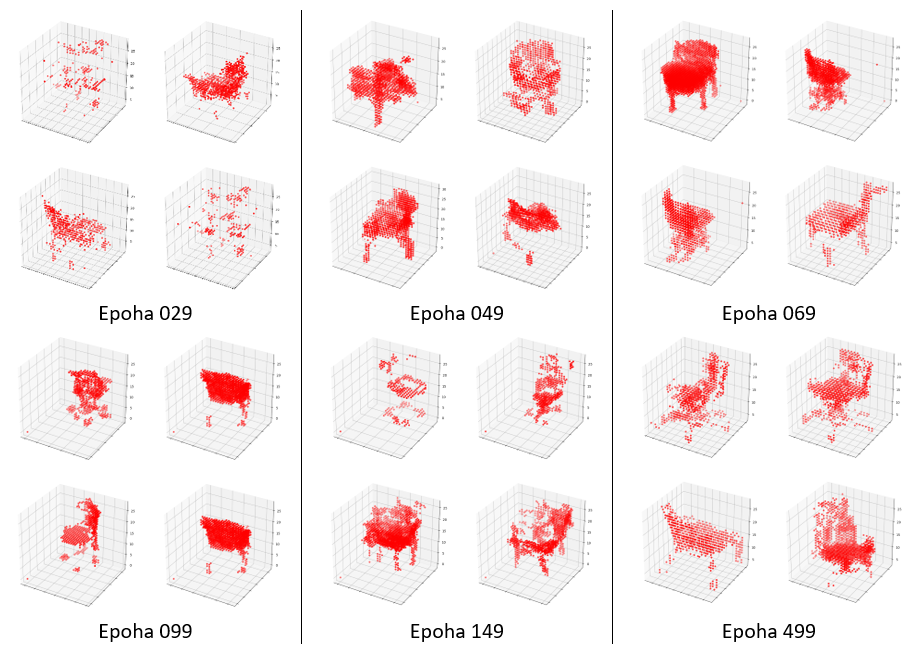
\includegraphics[width=1\linewidth]{32_200.png}
   \label{fig:Ng1} 
    \caption{32x32x32}
\end{subfigure}

\begin{subfigure}[b]{1\textwidth}
   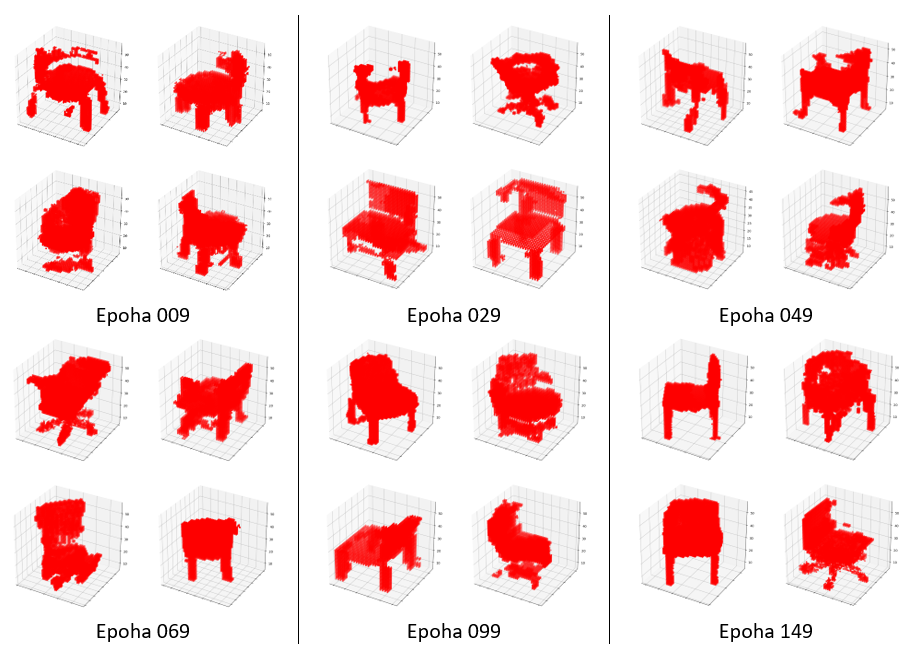
\includegraphics[width=1\linewidth]{64_400.png}
   \label{fig:Ng2}
   \caption{64x64x64}
\end{subfigure}
\caption{Uzorci modela tijekom treniranja}
\end{figure}

\break

\begin{figure}[h]
\centering
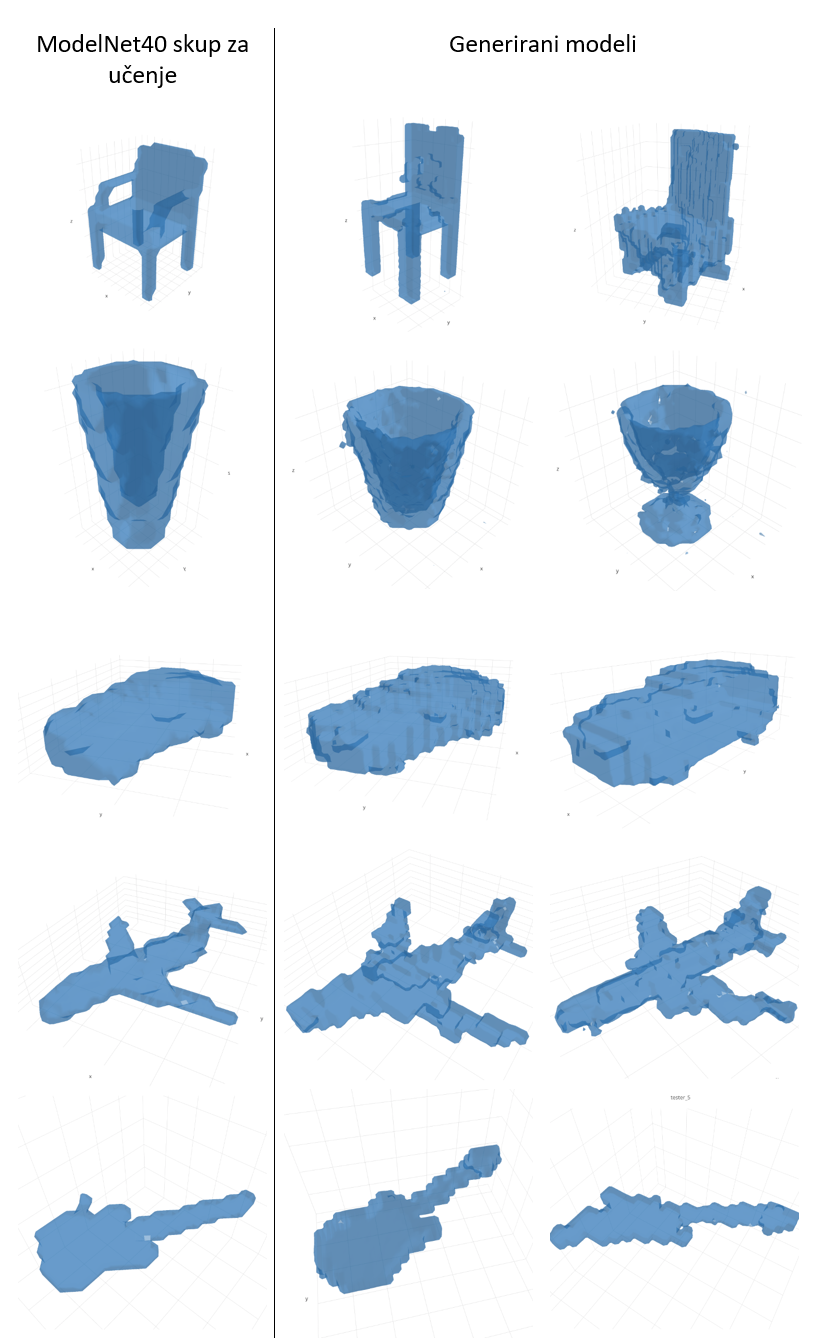
\includegraphics[scale=0.65]{primjeri.png}   
\caption{Usporedba generiranih objekata sa stvarnima}
\end{figure}

\clearpage

\begin{figure}[h]
\centering
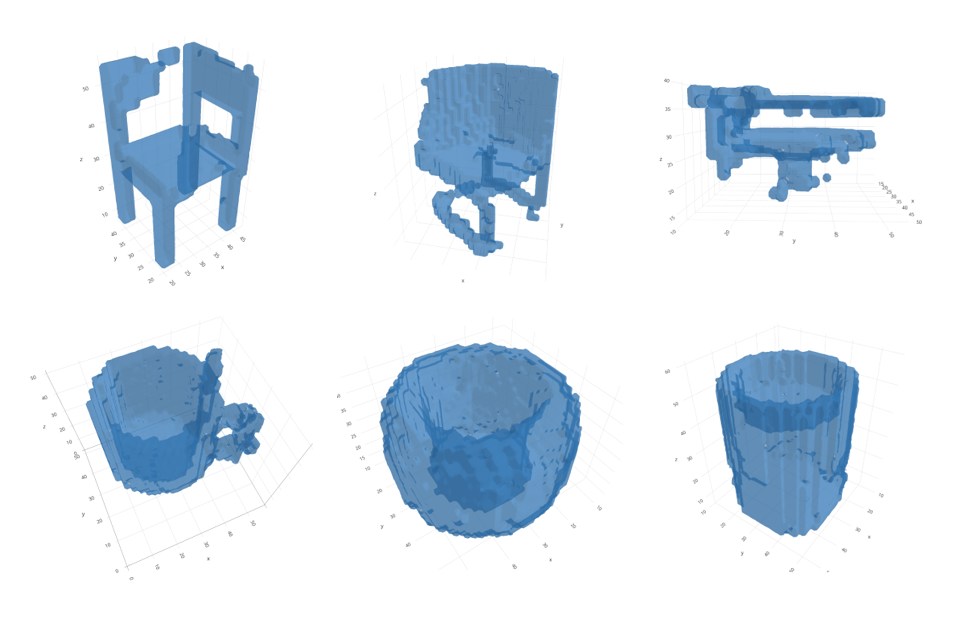
\includegraphics[scale=0.6]{primjeri_weird.png}   
\caption{Generirani objekti}
\end{figure}

\section{Generiranje ultrazvučnih slika pukotina}
Generiranje blokova pukotina u materijalu značajno je računalno zahtjevnije, zato što radimo s objektima dimenzija 128x128x128. Kod treniranja s originalnim 3DGAN parametrima, gubitak diskriminatora bi oko 100. epohe počeo padati prema 0, time vrlo brzo povećavajući pogrešku generatora, te bi se izgubila mogućnost poboljšanja generativnih sposobnosti daljnjim učenjem. S ažuriranim stopama učenja dobiveni su zadovoljavajući rezultati. Slika 6.6 prikazuje presjeke blokova generiranih primjera, izdvojenih algoritmom opisanim u odjeljku 5.4. Za usporedbu su prikazani presjeci stvarnih pukotina na slici 6.5. Ovime pokazujemo kako se generativni modeli mogu koristiti za povećavanje skupova za učenje klasifikacijskih mreža za prepoznavanje pukotina na ultrazvučnim slikama materijala, gdje mogu biti korisni kada nema dovoljno primjera za učenje mreže.

\begin{figure}[h]
\centering
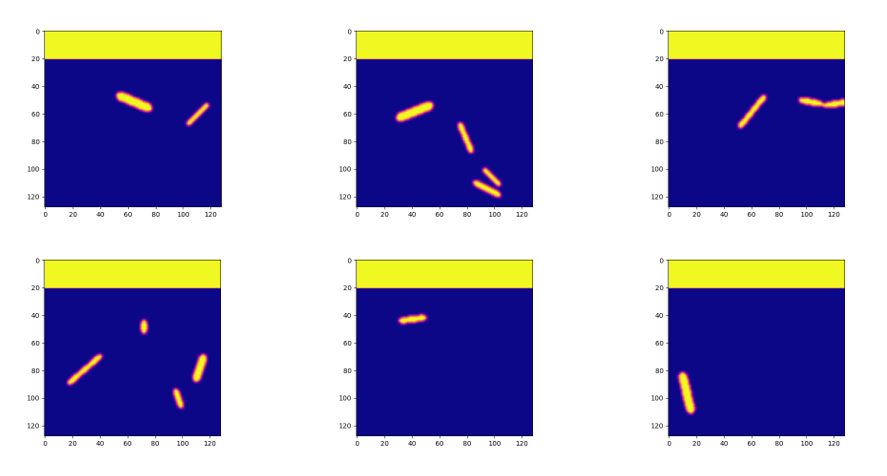
\includegraphics[scale=0.6]{dataset_6plot.png}   
\caption{Presjeci stvarnih primjera}
\end{figure}

\begin{figure}[h]
\centering
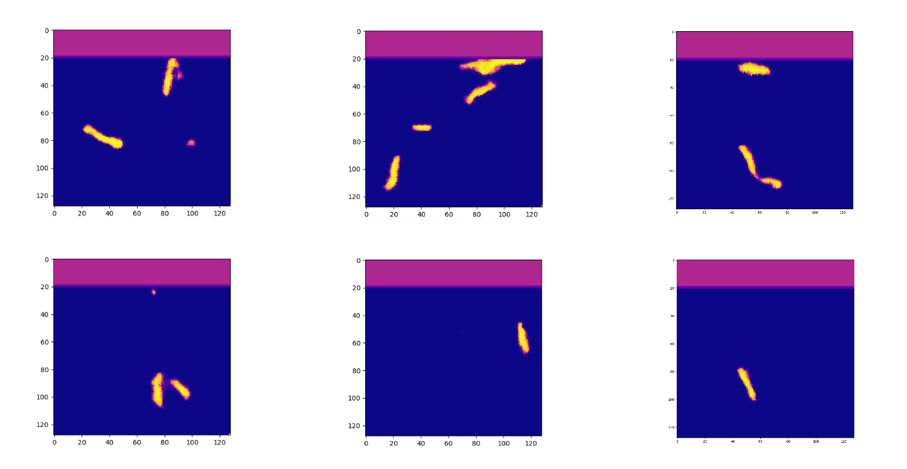
\includegraphics[scale=0.6]{generated_6plot.png}   
\caption{Presjeci generiranih primjera}
\end{figure}

\chapter{Zaključak}
Generativni modeli neuronskih mreža, a i područje dubokog učenja u svojoj cijelosti, iznimno se brzo razvijaju posljednje desetljeće. Iako se vodi rasprava jesu li naši pojednostavljeni modeli neurona i neuronskih mreža dovoljni da simuliraju kognitivne mogućnosti mozga, rezultati koje ove mreže postižu su zapanjujući, a u nekim primjenama i nadilaze naše sposobnosti, ponajviše zbog mogućnosti računala da obrade velike količine podataka u malo vremena.

Generativni modeli osobito su zanimljivi upravo zato što nisu diskriminativne prirode, nego kreiraju nešto do sad neviđeno. Njihovi različiti tipovi sposobni su sintetizirati primjere koji odgovaraju određenoj raspodjeli primjera za učenje, do te mjere preciznosti da mogu generirati ljudska lica koja ne možemo razlikovati od stvarnih.

Problem generiranja trodimenzionalnih objekata po mnogim je obilježjima složenija inačica generiranja dvodimenzionalnih slika i također znatno napreduje zadnjih godina. U ovom radu pokazana je točnost do koje arhitektura 3DGAN može generirati objekte rezolucije 64x64x64, veće nego prethodni radovi, te je primijenjena na problem generiranja ultrazvučnih slika pukotina u materijalu, s povećanom rezolucijom od 128x128x128. Pokazano je kako generiranje sintetskih slika može biti korisno u područjima gdje je problem dostupnost veće količine slika pa ih je za metode strojnog učenja potrebno generirati.


\nocite{simple}
\bibliography{literatura}
\bibliographystyle{unsrt}
%\bibliographystyle{fer}

\begin{sazetak}
Kod složenih modela dubokog učenja pojavljuje se problem nedostatka dovoljnog broja primjera za učenje. Moguće je poboljšati svojstva tih modela tako da se generiraju sintetski primjeri pomoću složenih modela generativnih suparničkih mreža. Ti modeli se brzo razvijaju i postaju sve sposobniji generirati realistične slike i modele. 3DGAN arhitektura omogućuje generiranje 3D modela veće preciznosti. U ovom radu je pokazana primjena te mreže na generiranje ultrazvučnih slika pukotina u materijalu, kako bi se povećanjem skupa primjera poboljšala generalizacijska svojstva mreža za klasifikaciju tih pukotina.

\kljucnerijeci{generativni suparnički modeli, neuronske mreže, umjetna inteligencija, strojno učenje, detekcija pukotina}
\end{sazetak}

% TODO: Navedite naslov na engleskom jeziku.
\engtitle{Models for generating three-dimensional objects}
\begin{abstract}
Complex deep learning models sometimes face the problem of not having enough learning examples. By generating synthetic examples with generative adversarial networks, it is possible to improve the capabilities of those networks. Those models are rapidly evolving and becoming more and more capable of generating realistic images and models. 3DGAN architecture makes it possible to generate 3D models of greater accuracy. This thesis shows the application of that network for generating ultrasound images of defects in materials, so that by enlarging the training set, we could improve the network's generalisation capabilities for classification of defects.

\keywords{Generative Adversarial Nets, Neural Networks, artificial intelligence, machine learning, detection of defects}
\end{abstract}

\end{document}
